\documentclass[10pt,twoside]{report}

\usepackage[utf8]{inputenc}

\usepackage[dvipsnames]{xcolor}

\usepackage{graphicx}
\graphicspath{ {images/} }

\usepackage[a4paper,width=150mm,top=25mm,bottom=25mm,bindingoffset=6mm]{geometry}

\usepackage{fancyhdr}
\pagestyle{fancy}

\usepackage{soul}
\newcommand{\hlc}[2][yellow]{ {\sethlcolor{#1} \hl{#2}} }

\usepackage[numbers]{natbib}
\usepackage{color}

\usepackage{amsmath}
\usepackage{amsfonts}

\usepackage[ruled]{algorithm2e}
\usepackage{multicol}

\usepackage{tikz}
\usetikzlibrary{shapes.geometric, arrows}

\usepackage{etoolbox}
\apptocmd{\sloppy}{\hbadness 10000\relax}{}{}

\usepackage{caption}
\usepackage{subcaption}

\newcommand{\ys}[1]{{\color{red} \bf[YS: #1 ]}}

\title{
    {Dynamic Resource Allocation for Multi-Camera Systems}\\\vspace{1cm}
    {\includegraphics[width=0.5\textwidth]{UvA-logo}}
}
\author{Eugenio Bargiacchi}
\date{\today}

\begin{document}

\maketitle

%\chapter*{Abstract}
%\chapter*{Dedication}
%\chapter*{Declaration}
%\chapter*{Acknowledgements}

\tableofcontents

\chapter{Introduction}\label{ref:intro}
%\item multi-sensor systems are everywhere. ex ....

With the advent of cheap hardware, these last few years have brought an incredible widespread
adoption of multi-camera systems. These systems are used for surveillance, real-time tracking and
many other purposes. Deployment expenses of such systems have progressively decreased with the
advent of digital multiplexing, the Internet and new manufacturing techniques. At the same time the
cost for operating the cameras and storing/analyzing the incredible amount of data they provide has
been increasing ever since. This often results in a need to operate multi-camera systems within
tight constraints, caused by both budget and technological limitations. Some such constraints can
be:

%\item they have resource constraints sometimes , ex ....

\begin{description}

\item[Limited Sensor Range:] Generally it is impossible for sensors to perceive simultaneously the
    whole environment in which they are located. This can result from a limited number of available
    sensors and/or from sensors having physical limits in what they can record. This constraint
    makes environments partially observable.

\item[Energy, Bandwidth and Communication Restraints:] Gathering and processing information consumes
    resources. Not only energy and bandwidth are expensive, but in many applications there are hard
    limits on their availability, both for what can be used at any given time and for the overall
    resource usage. This constraint forces information gathering from a subset of available sensors.

\item[Environment Size:] Camera systems are often deployed in order to provide surveillance
    facilities over large terrains or buildings. As the space that needs to be observed increases, the
    data that needs to be processed increases too. This constraint also limits the number of sensors
    that can be used at any one time, although the dependency here is more on the type and precision
    of the analysis performed on the data rather than a tight limit.

\end{description}

%\item in such cases, the goal of the agent is to reason about the constraint and minimize uncertainty about future,
%\item since these systems observe highly dynamic scenes (ex ... multi-camera systems), it is critical to reason about long term consequences

In order for such a multi-camera system to perform optimally within real world limits there is a
need to operate its sensors in an intelligent way, so to extract the most information with the
minimum cost while observing the aforementioned constraints. In particular, since multi-camera
systems are often deployed in highly dynamic contexts where targets can move rapidly between tracked
locations, there is a need to predict effectively the long-term evolution of the state of the
environment. This can be done by implementing an agent which will reason about the system's
dynamics and employ available resources in the best way.

At the same time, the agent needs to act while facing direct uncertainty about the environment it is
trying to observe. Reasoning with uncertainty is not a trivial task, given that the agent cannot
know in advance what knowledge will be obtained by a specific actions. Given only a certain
\textit{belief} on the current state of the environment and probabilistic expectations over the
amounts of information that will be extracted by each available action, the agent needs to reason so
to maximize the information gathered in the future.

%\item generally collecting information is not an means to an end , but in the example we gave above
% the aim of the agent is only to perceive the information. these type of tasks are called active
% perception task, define active perception. .....

The problem the agent faces falls under the \textit{Active Perception} \cite{cit:relworkspaan}
\cite{cit:relworkspaancoop} \cite{cit:relworksatsangi} task.  Active Perception can be formalized as
a task where a decision making entity called \textit{agent}, subject to resource constraints, needs
to take actions in order to reduce some form of uncertainty about a particular target environment.
The agent's role in this task is purely observational: it will not influence the overall evolution
of the environment over time, but it can only selectively gather data to maximally improve its
knowledge.

% \ys{this would be a good place to introduce the running example - surveillance task}

In this work we approach a surveillance task as an Active Perception problem: our goal is to produce
an agent system which will be able to track as best as possible a target moving through a partially
observable environment. The agent will need to exploit its available resources to determine the
target position over time. The agent will need to reason about the movements of the target even when
not observed, and use available cameras to observe the environment to refine as much as possible its
estimates over time.

%\item pomdp provide a natural framework to model such problems.

Active Perception tasks can be conveniently modeled through a powerful and flexible
decision-theoretic tool, called Partially Observable Markov Decision Process (POMDP)
\cite{cit:pomdp}. POMDPs provide a natural framework to model the interactions between the agent and
a partially observable, stochastic environment.  In the POMDP framework the agent's objective is to
maximize reward collection over time according to a predefined reward function.

POMDPs naturally allow for the computation of non-myopic strategies when reasoning over time is
required, as they are specifically structured as to allow this type of planning. This allows the
agent to gather information in order to improve its expected knowledge of the environment in the
future, while reasoning about all possibilities. We argue that while myopic strategies can sometimes
suffice, many Active Perception problems require non-myopicity to achieve optimality, and provide a
proof by example in Appendix \ref{ref:appendix_proof}.

% \ys{proof is a big word, generally they are associated with theorems, which we are not presenting. You can say a appendix provides convincing example case.}
%
% Eugenio: It actually is a proof (by example). So I am correct in stating it to be a proof. I've
% added the "by example" part.

% I think you should start by saying that you solve the surveillance problem (hopefully you introduce
% the surveillance problem somewhere in introduction) using online planning.
% ----------------
% I think you should motivate online planning
% here on the idea that as the size of the system increases, it is difficult to use offline methods

POMDPs are a widely explored topic in the decision theoretic literature, with known properties and
already available solution methods. In particular, our approach is based on online planning
\cite{cit:relworkonlineall}. This type of approach is based on determining an optimal course of
action applicable only to the situation that is currently faced by the agent, ignoring the others.
Online planning requires reasoning continuously over time, but it is simpler to perform as the size
of a problem increases than offline methods, which tackle the whole problem at once beforehand.

% You use MCTS to solve the problem. ... we use MCTS because of better performance

In this work we approach the surveillance problem by extending one of the fastest online Monte Carlo
planners for POMDPs, Partially Observable Monte Carlo Planning (POMCP) \cite{cit:pomcp}. This
method approximates beliefs about the world using particles, improving performance when the
maintaining a complete belief over the state of the world can become too computationally expensive.

The limitation of POMCP with respect to the Active Perception task is that the algorithm evaluates
actions using rewards which depend on the state of the environment. Unfortunately, such evaluation
cannot take into account the knowledge of the agent, and thus results useless to compute a good
policy for the agent when it needs to maximize its knowledge. POMDPs where rewards are based on
knowledge, rather than state, have been examined in \cite{cit:rpomdp}.

% You propose a new variant of MCTS, suitable for belief-dependent rewards leading to better
% estimates/performance.

We extend POMCP and create a variant, which we named $\rho$-POMCP, which is able to deal with a
reward function based on knowledge rather than state. Our solution is able to refine estimates of
action rewards from the imperfect particle beliefs of POMCP. This allows to apply a fast online
planner on Active Perception tasks.

% Finally we illustrate empirical success of our method.

We show empirical tests and performance of our method on a number of problems which show the
effectiveness of our method with limited resources and its ability to scale with the size of the
problem with respect to already available methods.



\chapter{Background}\label{ref:background}
\section{Partially Observable Markov Decision Process}\label{ref:pomdp}
\sectionmark{POMDP}

The \textit{Partially Observable Markov Decision Process} (POMDP) \cite{cit:pomdp} is a framework
which allows to model the dynamics of an environment in order to produce a policy that fulfills a
given task. POMDPs structure reasoning around a probabilistic automaton \cite{cit:probautomata}. An
agent \textit{acts} upon the environment, which is in a particular \textit{state}. As a result, the
environment \textit{transitions} stochastically to another state, as defined by a transition
function. During the transition, the agent receives a certain \textit{reward} representing its
achievements toward the task at hand.

In a POMDP the agent cannot see directly the current state of the world. Instead, the agent receives
an \textit{observation} dependent on the underlying state during each transition, which may or may
not uniquely disambiguate it. The observations are used to keep a statistic over the states the
environment could be in at any given time.

The objective of the agent is to maximize the reward obtained by acting in the environment while
reasoning about the state uncertainties. In doing so it will accomplish the task that is encoded
within the POMDP model.

% \ys{transition function can be subsubsection ?? and so can be other bullets. }
%
% Eugenio: Shimon told me he didn't like too many subsections (before I had a subsection for each
% component of the POMDP - T, R, O, and so on..). So I'm not sure what to do. I've removed the old
% subsections, maybe I'll ask Shimon directly what subsections he would like so I can do it once and
% for all.
%
% \ys{bullets are fine. No need to change.}
%
% It's ok, but I guess I'd rather wait for Shimon to say how he prefers to structure this so we can
% all be on the same page.
%
A POMDP is defined as a tuple

\begin{equation}
 POMDP = <S,A,T,R,\Omega,O,h>
\end{equation}

The elements of the tuple are called \textit{state space}($S$), \textit{action space}($A$),
\textit{transition function}($T$), \textit{reward function}($R$), \textit{observation
space}($\Omega$), \textit{observation function}($O$) and \textit{horizon}($h$).

The state space contains all possible configurations the environment can take.  The environment
transitions between states discretely and instantaneously at each \textit{timestep}, which
represents the atomic unit of change within the environment.

\begin{equation}
 S = \{s_0, s_1, s_2, ..., s_{|S|}\}
\end{equation}

All states must have the \textit{Markov} property, which means that the evolution of the environment
must depend solely on the information encoded in its current state, and nothing else. The Markov
property is required in order to allow the agent to reason only about the current state, which makes
POMDPs tractable.

The action space contains all actions available to the agent. Each action simultaneously fulfills
two purposes: to influence the evolution of the environment, and to gather information regarding the
state of the environment.

\begin{equation}
 A = \{ a_0, a_1, a_2, ..., a_{|A|} \}
\end{equation}

The observation space contains all observations that the agent can receive from the environment; at
each timestep the agent receives a single observation from the environment which is dependent on
the action performed and the new state of the environment.

\begin{equation}
 \Omega = \{ o_0, o_1, o_2, ..., o_{|\Omega|} \}
\end{equation}

The transition function encodes the consequences of actions with respect to the environment states.
It specifies the probability that by performing an action $a$ in a state $s$, the
environment will transition to a new state $s'$.

\begin{equation}
 T(s, a, s') = Pr(s' | s, a)
\end{equation}

Where $Pr(s'|s,a)$ is the probability of the environment transitioning to $s'$ from $s$ when the
agent performs action $a$. By using this notation, we can show formally what the Markov property is
about. This property holds when

\begin{equation}
 Pr(s_{t+1} | s_{0}, a_{0}, s_{1}, a_{1}, ..., s_{t}, a_{t} ) = Pr(s_{t+1} | s_t, a_t ) \hspace{1cm}
 \forall s \in S \wedge \forall a \in A
\end{equation}

where $t$ denotes the timestep where a particular state was reached.

The observation function represents the probability of obtaining a certain observation upon reaching
a given state $s'$ after taking action $a$.

\begin{equation}
 O(s', a, o) = Pr(o | s', a)
\end{equation}

Note that the state is the one of \textit{arrival}, not the one where the action is performed.

The agent goals are encoded within the reward function. This function is defined upon states and
actions, and can take values within the real domain:

\begin{equation}
 R(s, a, s') \in \mathbb{R}
\end{equation}

The reward function represents the level of appeal that a particular situation or outcome represents
in the modeled task. For example, one could allocate a certain reward for using a camera, and an
even greater reward for successfully finding the current location of the target. This would result
in the agent actively pursuing those goals. On the other hand, one could allocate a negative reward
for failed tracking attempts, to prevent a mindless use of limited resources.

Finally, the horizon specifies for how many timesteps the agent is allowed to act on the
environment. The agent will then find the best strategy in order to maximize accrued reward within
this time constraint.

We can make a brief example of how the POMDP framework works within the context of multi-camera
tracking of a single target. The state space would be represented by each possible state of the
environment, thus each state would represent a possible location of the target. At each timestep,
the agent would take a single action, to guess the current position of the target and to collect a
noisy observation from a subset of the cameras available to it. At the same time, the target would move
to a different location, as specified by the transition function. In this problem the transition
function is independent of the action of the agent, since looking through a camera has no effect on
the movement of the target.

The observation would be collected with respect to the new position of the target and the camera
chosen by the agent, as specified by the observation function, which would also model input noise.
The agent would also collect a reward depending on its guess of the previous position of the target.
The process would then repeat for each remaining timestep.

% \ys{Why is this model in background? when explaining the model, explain why only one camera can be chosen at each time step?}
%
% It's more like the example we agreed to put in? We said to have a recurring example and to use it,
% so I explained POMDPs with the example. I've removed the only one camera part though, that
% should not have been there.

\subsection{History and Belief}

The observation function does not allow the agent to disambiguate between states unambiguously.
Instead, what happens is called \textit{perceptual aliasing}: each obtained observation is
compatible with a subset of $S$.

The agent must reason about which of the possible underlying states of the environment are
compatible with all previously obtained observations in order to plan its moves.

Unfortunately, this requires the agent to remember the past to reason effectively. While the
environment states maintain their Markov property, which would allow the agent to ignore previous
events, the agent cannot observe them. Instead it needs to store internally its whole history of
actions and observations in order to keep track of which states are possible at any point during an
episode. This long list of actions and observations is called \textit{history}.

An alternative way of maintaining the history is keeping a \textit{belief} over the current state of
the environment. Such a belief is simply a probability vector in $|S|$ dimensions, where each
element denotes the probability that the environment is in a particular state. The belief is a
\textit{sufficient statistic} of the state of the environment \cite{cit:pomdp}.

At each new timestep, the agent's belief needs to be updated with the new knowledge gained by the
agent. The belief can be updated with the following formula:

\begin{equation}
 b'(s') = \frac{O(s', a, o)\sum_{s\in S}T(s,a,s')b(s)}{Pr(o|a,b)}
\end{equation}

The denominator can be treated as a normalizing factor that makes $b'$ correctly sum up to 1, since
it is a probability vector.

The belief allows for a reinterpretation of the POMDP framework. The belief can in fact be used in
lieu of a state, since it is possible to compute new transition and reward functions that depend on
beliefs rather than states. This transforms automatically the POMDP into a \textit{belief MDP}
\cite{cit:pomdp}, where the belief is now the state of the environment. An MDP
\cite{cit:suttonbarto} is a subset of POMDPs, where the agent always knows the state of the
environment and thus requires no observations.

The belief MDP is created by generating a new transition function $\tau$ and a \textit{belief
dependent reward} function $\rho$ as follows:

\begin{equation}
 \tau(b,a,b') = \sum_{o\in \Omega} Pr(b' | b, a, o) \sum_{s\in S} O(s,a,o) b(s)
\end{equation}

Where

\begin{equation}
Pr(b' | b, a, o) = \left\{
  \begin{array}{lr}
    1 \hspace{.6cm}\text{if the belief update with arguments $b,a,o$ returns $b'$}\\
    0 \hspace{.6cm}\text{otherwise}
  \end{array}
\right.
\end{equation}

Similarly:

\begin{equation}
 \rho(b,a) = \sum_{s\in S} R(s,a) b(s)
 \label{rhoeq}
\end{equation}

Although this transformation allows us to forget the partial observability, which is now embedded in
$\tau$, we have now introduced a new problem: a continuous state space. Although continuous MDPs are
very hard to solve generally, the belief MDP can be approached due to its specific properties, which
will be discussed shortly.

\subsection{Policy}

In the POMDP framework the agent tries to maximize its \textit{expected return} within an
\textit{episode}: the expected sum of all rewards obtained within a single try at the task.

The length of a specific episode is determined by a parameter called \textit{horizon}. An horizon of
1 timestep generates what is generally known as a \textit{myopic policy}. Such a policy acts in a
locally optimal way, hoping that in doing so it will act in an optimal way globally. As the horizon
increases the final policy takes into account more and more possible outcomes, becoming more complex
but, depending on the task, more performant overall. We can describe the goal function of a POMDP
with finite horizon $h$ as:

\begin{equation}
 \mathbb{E}[\text{return}] = \mathbb{E} \left [ \sum_{t=0}^{h-1} R(s_t, a_t, s_{t+1}) \right ]
\end{equation}

A solution for a POMDP is called a \textit{policy}. We can define a policy $\pi$ as a function, that
given an horizon, a belief and action returns the probability of the action being chosen:

\begin{equation}
 \pi : H \times B \times A \rightarrow [0,1]
\end{equation}
\begin{equation}
 \pi(h, b, a) \in [0,1]
\end{equation}

We can also define it as a function, taking a belief and an horizon, returning a distribution over
actions:

\begin{equation}
 a \sim \pi(h, b)
\end{equation}

A policy performance can be evaluated through a \textit{value function}. The value function maps a
policy with its performance in terms of expected return from every possible belief the agent may
face and a particular horizon. Thus, every belief has a certain \textit{value} under a certain
policy and horizon. Formally then we can define the value of a belief as:

\begin{equation}
 V^\pi_{h}(b) = \mathbb{E}^\pi_h \left [\text{return} \mid b_0 = b \right ]
\end{equation}
\begin{equation}
 = \mathbb{E} \left [\sum_{t=0}^{h} \rho(b_{t}, a_t, b_{t+1}) \right ]
    \hspace{0.5cm}\text{where }b_0 = b \text{ and }a_t \sim \pi(h-t, b_t)
\end{equation}

This value is very important because it lets us compare and evaluate policies. This is because a
better policy does have a equal or higher value for every possible belief than an inferior policy
\cite{cit:suttonbarto}.

A value function can be expressed recursively with the \textit{Bellman equation}. This equation
states that the value of a state can be computed as the expected reward that the agent can obtain in
the next timestep, plus a value which represents what is going to happen in the future.

\begin{equation}
 V^{\pi}_{h}(b) = \sum_a \pi(h, b, a) \sum_{b'} \tau(b, a, b') \left [ \rho(b, a, b') +
V^{\pi}_{h-1}(b') \right ]
\end{equation}

Since the value function of a POMDP is a function dependent on beliefs, it is defined on a simplex
space of $|S|-1$ dimensions, which is continuous. The property that makes a belief MDP tractable is
that its value function is \textit{piecewise linear and convex} (PWLC) \cite{cit:pomdp}. This means that it is
``determined by a set of hyperplanes, the value at a given belief point being that of the highest
hyperplane'' \cite{cit:rpomdp}. An example of this property is shown in Figure \ref{pwlcpic}. This
makes it possible to solve a belief MDP exactly, since the optimal policy is finitely bounded in the
number of components it is made of \cite{cit:pomdp}.

\begin{figure}[ht]
\begin{center}
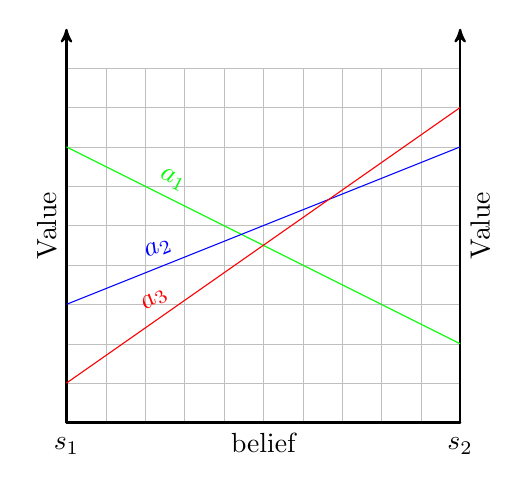
\begin{tikzpicture}[>=stealth',auto,node distance=4cm,main node/.style={circle,draw,font=\Large\bfseries}]
\tikzstyle{state} = [circle, draw=black, fill=green!30]

\node[] at (0,-0.3) {$s_1$};
\node[] at (5,-0.3) {$s_2$};
\draw[step=0.5cm,lightgray,ultra thin] (0,0) grid (5,4.5);
\draw[thick, line cap=round] (0,0) -- (5,0) node[midway, anchor=north] {belief};
\draw[thick,->, line cap=round] (0,0) -- (0,5) node[midway, anchor=south, rotate=90] {Value};
\draw[thick,->, line cap=round] (5,0) -- (5,5) node[midway, anchor=north, rotate=90] {Value};
\draw[green] (0,3.5) -- (5,1) node[near start, anchor=south, sloped] {$a_1$};
\draw[blue] (0,1.5) -- (5,3.5) node[near start, anchor=south, sloped] {$a_2$};
\draw[red] (0,0.5) -- (5,4) node[near start, anchor=south, sloped] {$a_3$};

\end{tikzpicture}
\end{center}
\caption{An example of the PWLC property of the value function for a two state POMDP. Each line
represents an \textit{alpha vector}, which represents the value of a possible sequence of action in
any given possible belief. The value of the optimal policy is represented by the max of all possible
alpha vectors at any belief point, and thus is composed of a finite amount of linear components,
arranged in a convex shape.}
\label{pwlcpic}
\end{figure}

In general, when we are looking for a solution for a POMDP we are looking for a policy $\pi^*$, called
\textit{optimal policy}, that maximizes the value over all beliefs:

\begin{equation}
 V^{\pi^*}_h = \max_\pi V^{\pi}_h
\end{equation}

Another useful function that can be defined from $V$ is the value of a given action $a$ in a
particular belief, given that the specified policy is strictly followed after taking $a$:

\begin{equation}
 Q^{\pi}_h(b, a) = \sum_{b'} \tau(b,a,b') \left[ \rho(b,a,b') + V^{\pi}_{h-1}(b') \right ]
\end{equation}

The \textit{Q-Function} is extremely useful since the optimal policy can be easily extracted from
it, simply by selecting at each belief the action that maximizes it. This work leverages this fact
by approximating the Q-function and then extracting the optimal policy from it.

\section{$\rho$POMDP}\label{ref:backrpomdp}

As we have already mentioned, in a belief MDP the reward is defined in terms of the belief and the
normal reward function $R$, as shown in Equation \ref{rhoeq}.

However, in some cases the reward function is solely dependent on the information the agent has on
the current state of the world, rather than on the underlying state of the world itself. In such
situations the original POMDP reward function becomes useless, together with our definition of
$\rho$.  For example, in the case of surveillance, there is no inherent reward for the agent when
the environment is in a state rather than another. Instead, the agent actions should maximize the
knowledge that the agent has of the world.

% \ys{There is no need to motivate active perception in background. Describe $rho$POMDP here.}
%
% It's true that this is a motivation, but I guess it also introduces the reasoning for rhoPOMDPs,
% which I guess could be useful.. half the sentence is an example, which we said was good to use in
% the thesis. If it turns out that it "weights" the thesis too much I'll remove it, no worries.

In such cases the $\rho$ function is defined independently, and is not tied to states anymore. The
resulting framework is a variant of POMDP, called $\rho$POMDP, where $\rho$ substitutes $R$, while
all other elements of the original POMDP stay the same.

In the $\rho$POMDP framework unfortunately the PWLC property of the value function does not hold
anymore, and so the solving methods which rely on it cannot be used. While it has been proved in
\cite{cit:rpomdp} that as long as the newly defined $\rho$ function is PWLC then the value function
will be PWLC as well, functions such as entropy are not PWLC in the first place. 

A possible solution is outlined in \cite{cit:pomdpir}: it is possible to approximate $\rho$ via a state-based reward function, by extending the action space with \textit{prediction actions}. The agent can use prediction actions to explicitly guess the underlying true state of the environment, gaining reward when correct. Thus, these additional actions have the effect of rewarding the agent for information gain, since if it is able to assert with a high degree of certainty the underlying true state of the environment it will be able to obtain a higher reward. Prediction actions are taken alongside the normal actions, resulting in an action space which is the cross-product of normal actions and prediction actions. The resulting approximated value function is PWLC, at the expense of a more complex POMDP that needs to be solved.

Our approach, which we discuss in Section \ref{ref:approach}, is different, and relies on the properties of a particular class of solving techniques, but we compare against this approach in Section \ref{ref:experiments}.

% \ys{you should explain $\rho$POMDP here. What you have written here, does not even talk about what $\rho$POMDP is. It only outlines the problem which $\rho$POMDP solves.}
%
% Eugenio: I'm not sure I understand. As we have already said multiple times, \rhoPOMDP is the
% framework which replaces R with \rho. Thus I fell I have explained here adequately what it is
% (since it is relatively easy to explain after all).


\section{Planning vs Reinforcement Learning}\label{ref:solutions}

While often the possible states, actions and observations of a particular environment are easy to
define, it does not always happen that the transition, observation and reward functions are known in
advance.

When they are known, the solving process is called \textit{planning}, and consists in efficiently
looking through all possible transitions the agent could experience, and finding the best path
through them in order to maximize the return.

On the other hand, when they are not known, \textit{reinforcement learning} is used. In this case the
focus is on gathering knowledge about the environment while \textit{at the same time} exploiting that
knowledge to obtain the maximum return. Reinforcement learning methods can range from approximating
the unknown functions from experience and then planning, to approximating the optimal value function
of the model and using it to obtain a policy, or even directly approximating the optimal policy.

In this work we assume we are either given a model, or a model is learned in advance, and that this
model is used as a base for planning.

\section{Offline vs Online}

An optimal policy can be applied at virtually no computational cost with the knowledge that the
behavior is constantly optimal. Computing such a solution in advance and using it later is called
\textit{offline planning}. The main disadvantage of offline planning is its very heavy upfront cost:
it needs to store all possible policies to be applied to any reachable belief at any horizon. This
is expensive not only in terms of space, but even more on computation, since any non-trivial POMDP
has an exponential explosion in the number of possible histories that an agent can experience and
each one of them has to be considered in order to evaluate the final policy \cite{cit:pomdp}. In
addition, any small change in the original model requires a full recomputation of the optimal
policy, which limits the amount of tuning that can be feasibly done on the model.

Offline planning methods generally leverage the Bellman equation and the recursive nature of the
value function; they plan in reverse temporal order, from the last steps the agent will take to the
first ones. This is because a policy for a certain horizon $h$ is always composed by a set of
actions to apply in certain beliefs which then leads to a policy for horizon of $h-1$. Thus, the
final policy needed is computed incrementally. All possible state, actions and observations are
considered, so as to provide the correct action in every possible situation.

In order to avoid the computational cost of offline methods, a new venue of approach was invented
called \textit{online planning}. In online planning the agent continuously plans for its current
belief, and nothing else. This requires constant computations, but at the same time makes possible
to tackle problems orders of magnitude bigger than what is possible with offline planning, and allow
for flexibility in updating the model, since there is no need to recompute a complete solution. In
addition, many online planning methods are \textit{any time}: this means that they can run for
whatever time is available, and they are always able to provide some sort of solution. The more time
is available, the more refined the solution will be. This is in contrast with offline methods, that
need to run to completion or otherwise nothing is gained.

In online planning computations go forward in time. From the current state possible futures are
expanded in a tree of possibilities and rewards. In the end, the best action for the current state
is picked, the environment is advanced one step, and the process repeats again.

In this work we chose to use an online approach, given the flexibility and power provided over
offline techniques, and because one of our goals was to scale to real-world scenarios, which are
generally intractable with offline approaches. An additional advantage which we will explore later
is that online planners are able to deal with non-PWLC value functions, which is a challenge when
using negative entropy as a reward function.

\section{Monte Carlo Algorithms}

At the time of writing, one of the most promising ways of planning online is by using \textit{Monte
Carlo algorithms}. Monte Carlo algorithms are a class of randomized algorithms which use random
processes in order to compute their output. The output will be correct within a certain probability,
which trades off with their speed, deterministic running time and anytime properties.

In the MDP/POMDP frameworks Monte Carlo algorithms only need results from samples of the
environment; as in, transition and reward results sampled from the model's distribution using
particular state-action pairs as inputs. Such a model is also called a \textit{generative model}. A
generative model $G$ fed with state $s$ and action $a$ would return a new state $s'$ and reward $r$
respecting the model probabilities:

\[ s', r \sim G(s, a) \]

An advantage of using such a model is that it many cases it is possible to obtain samples without
having the whole transition function for the model in an explicit form. The samples obtained can
then be used to approximate average returns, which in turns can be used to obtain an optimal policy.

\section{Monte Carlo Tree Search}

The most widely known algorithm using Monte Carlo techniques is called \textit{Monte Carlo Tree
Search} (MCTS) \cite{cit:mcts}. This algorithm is an MDP online planner which has received high
praise for its contributions in the development of highly performant board game AIs.

MCTS was originally devised as a method to approach the board game Go. The algorithm runs Monte
Carlo simulations from the current state, which is the input, and progressively builds
a tree of outcomes.

\begin{algorithm}
\begin{multicols}{2}
    \caption{Monte Carlo Tree Search}
    \SetKwFunction{mcts}{MCTS}
    \SetKwFunction{simulate}{Simulate}
    \SetKwFunction{rollout}{Rollout}

    \SetKwProg{main}{Algorithm}{}{}
    \main{\mcts{s}}{
        \KwData{State s}
\nl     \While{enough time is available}{
\nl         \simulate{\O, s, 0}\;
        }
\nl     \KwRet most valued action in tree root\;
    }

    \setcounter{AlgoLine}{0}
    \SetKwProg{myproc}{Procedure}{}{}
    \myproc{\rollout{s, d}}{
        \KwData{State s, Depth d}
\nl     r = 0\;
\nl     discount = 1\;
\nl     \While{$d <$ horizon}{
\nl         ($s', r'$) $\sim$ G($s$, random action)\;
\nl         r = r + discount * $r'$\;
\nl         discount = discount * $\gamma$\;
\nl         $s$ = $s'$\;
        }
\nl     \KwRet r\;
    }

    \setcounter{AlgoLine}{0}
    \SetKwProg{simul}{Procedure}{}{}
    \simul{\simulate{h, s, d}}{
        \KwData{History h, State s, Depth d}
\nl     select action $a$\;
\nl     ($s', r$) $\sim$ G($s,a$)\;
\nl     \If{$d < $ horizon}{
\nl         \eIf{T($h,a,s'$) is not \O}{
\nl             futureRew = \simulate{$(h,a,s'), s', d+1$}\;
            }{
\nl             initialize T($h,a,s'$)\;
\nl             N($h,a$) = V($h,a$) = 0\;
\nl             futureRew = \rollout{s', d+1}\;
            }
\nl         r = r + $\gamma$ * futureRew\;
            }
\nl     N($h,a$) = N($h,a$) + 1\;
\nl     V($h,a$) += $\frac{r-V(h,a)}{N(h,a)}$\;
\nl     \KwRet r\;
    }

\end{multicols}
\end{algorithm}

The MCTS tree of outcomes starts out as a single root. This root represents the current state of the
agent. From this root MCTS carries out as many sample episodes as possible. After each sample
episode, the MCTS tree is expanded, keeping track of all possible futures experienced by MCTS.

Each sample episode can be divided into two phases: in the first the algorithm descends the
known tree, while in the second the algorithm simulates outside it.

Descending the tree is done recursively in a very simple fashion. Starting from the root node $s$, the
algorithm selects an action $a$, and uses both to produce a reward $r$ and a next state $s'$. The
action is selected probabilistically, with more promising actions selected more often.  The root
children are then searched for a node representing the sequence $(a,s')$. If one is found, the
algorithm descends one level in the tree, and repeats the action selection and sampling process,
this time using the last $s'$ as its $s$.  This repeats until the algorithm is unable to descend
further into the tree.

Once the bottom of the tree is reached, the algorithm adds a single child node to the reached leaf.
The node represents the $(a,s')$ from the last sample. Once this is done, MCTS enters its
second phase.

During the second phase the algorithm continues to simulate the episode, but it does not use the
tree anymore. Actions are selected using a \textit{rollout policy}, which is generally uniformly
random. This continues until a terminal state or the selected horizon is reached. This concludes the
sample episode.

Once a sample episode ends, all the reward collected during both phases is backpropagated up to the
tree root. This is used to update the values of all the actions taken during the first phase of the
algorithm.

At this point, a new sample episode is started from the root of the tree. This process is repeated
until there is time left.

A nice property of MCTS is that it is guaranteed to converge to the optimal policy as long as the
most promising actions are given a higher probability of being chosen than the others. This is
because in the long run the value averages will converge to the values of the actions taken most
often.  In addition, since it builds a tree, part of the work done can be reused on the next time
step. Once a move is tried in the real world, the tree root can be moved to the new state perceived,
while the rest of the tree is discarded.

\section{Upper Confidence Bounds for Trees}

A technique which has recently gained popularity to exactly determine which actions should be chosen
within the tree and which ratio should be used between promising actions and the rest is called
\textit{Upper Confidence Bounds for Trees} (UCT) \cite{cit:uct}. UCT tries to empirically derive a
variance estimate from the data, sorting actions by their upper bounds on value.

The upper bound estimate is composed of two parts: the currently estimated value of the action $v$,
and the estimated UCT variance. Thus the value that UCT assigns at a given action $a$ is:

\[ UCT(a) = v + c*\sqrt{\frac{\log{N}}{n}} \]

Where $N$ is the number of times the node in the tree currently being considered has been visited,
and $n$ is the number of times action $a$ has already been tried from the node. $c$ is a constant
which is dependent on the problem, which defines the amplitude of the variance, which needs to be in
tune with the magnitude of the rewards of the MDP. This number is generally tuned manually, and is
around the maximum return that can be obtained by the agent.

Actions are then selected greedily with respect to the UCT value.

\section[]{Partially Observable Monte-Carlo Planning%
\sectionmark{POMCP}}
\sectionmark{POMCP}

\textit{Partially Observable Monte-Carlo Planning}(POMCP) \cite{cit:pomcp} is one of the
state-of-the-art online solvers available today. This algorithm incorporates the advantages of MCTS
while adding support for belief states and observations.

The trouble of naively applying MCTS to a belief MDP extracted from a POMDP is its necessity to
sample directly from state to state. While this can be a cheap operation in MDPs, requiring
samples from relatively simple distributions, computing a new belief given a previous belief and
observation in a POMDP, called \textit{belief update}, can be a very expensive operation. Recall that a belief
update can be performed using the following formula:

\[ b'(s') = \frac{O(s', a, o)\sum_{s\in S}T(s,a,s')b(s)}{Pr(o|a,b)} \]

For a full belief, this requires $O(|S|^2)$ operations, which for POMDPs with a large state space
can result in an extremely expensive operation. Since MCTS requires a very high number of samples in
order to provide useful answers, each sample needs to be performed in as little time as possible,
and such expensive operations are thus not acceptable.

POMCP solves this problem by representing beliefs as particle vectors containing a certain amount of
state particles. Such a \textit{particle belief} can be created by repeatedly sampling a belief, and
gathering all samples in a vector - not a set.

\begin{algorithm}
    \caption{Partially Observable Monte-Carlo Planning}
\begin{multicols}{2}
    \SetKwFunction{pomcp}{POMCP}
    \SetKwFunction{simulate}{Simulate}
    \SetKwFunction{rollout}{Rollout}

    \SetKwProg{main}{Algorithm}{}{}
    \main{\pomcp{b}}{
        \KwData{Belief b}
\nl     \While{enough time is available}{
\nl         s $\sim$ b\;
\nl         \simulate{\O, s, 0}\;
        }
\nl     \KwRet most valued action in tree root\;
    }

    \setcounter{AlgoLine}{0}
    \SetKwProg{myproc}{Procedure}{}{}
    \myproc{\rollout{s, d}}{
        \KwData{State s, Depth d}
\nl     r = 0\;
\nl     discount = 1\;
\nl     \While{$d <$ horizon}{
\nl         (s', r') $\sim$ G(s, random action)\;
\nl         r = r + discount * r'\;
\nl         discount = discount * $\gamma$\;
\nl         s = s'\;
        }
\nl     \KwRet r\;
    }

    \setcounter{AlgoLine}{0}
    \SetKwProg{simul}{Procedure}{}{}
    \simul{\simulate{h, s, d}}{
        \KwData{History h, State s, Depth d}
\nl     select action $a$ with UCT\;
\nl     ($s', o, r$) $\sim$ G($s,a$)\;
\nl     \If{$d < $ horizon}{
\nl         \eIf{T($h,a,o$) is not \O}{
\nl             futureRew = \simulate{$(h,a,o), s', d+1$}\;
            }{
\nl             initialize T($h,a,o$)\;
\nl             N($h,a$) = V($h,a$) = 0\;
\nl             futureRew = \rollout{s', d+1}\;
            }
\nl         r = r + $\gamma$ * futureRew\;
            }
\nl     B(h) = B(h) $\bigcup \;\{ s' \}$\;
\nl     N($h,a$) = N($h,a$) + 1\;
\nl     V($h,a$) += $\frac{r-V(h,a)}{N(h,a)}$\;
\nl     \KwRet r\;
    }

\end{multicols}
\end{algorithm}

POMCP starts its execution in the root of the tree, which represents the current particle
belief of the agent. POMCP, as MCTS, is again composed of two phases: tree descent and outside tree
simulation. The procedures for both are very similar to the MCTS originals.

Starting from the root, POMCP samples a single state $s$ from the root's particle belief. Then,
using UCT, it selects a state $a$, and uses it with $s$ to sample a new state $s'$, a reward $r$ and
an observation $o$. The root children are then searched for a node representing the sequence
$(a,o)$. If one is found, the algorithm descends one level into the tree. While descending, POMCP
appends $s'$ to the particle belief of the selected child node. Then, it repeats the action
selection and sampling process using $s'$ as its $s$. This repeats until the algorithm is unable to
descend further into the tree.

The adding of particles to lower level particle beliefs is the way POMCP updates beliefs, without
the $O(|S|^2)$ complexity.

Once the bottom of the tree is reached, the algorithm adds a single child node to the reached leaf.
The node represents the $(a,o)$ from the last sample. It also adds to the new node's particle belief
its first particle, the final $s'$. Once this is done, POMCP enters its second phase.

During the second phase the algorithm continues to simulate the episode, but it does not use the
tree anymore. Actions are selected using a \textit{rollout policy}, and observations sampled are
completely discarded. This continues until a terminal state or the selected horizon is reached. This
concludes the sample episode.

Once a sample episode ends, all the reward collected during both phases is backpropagated up to the
tree root. This is used to update the values of all the actions taken during the first phase of the
algorithm.

At this point, a new sample episode is started from the root of the tree. This process is repeated
until there is time left.


\chapter{Approach}\label{ref:approach}
\section{$\rho$-POMCP}

As discussed, the POMCP algorithm can't be applied directly to $\rho$-POMDPs. In this Section we
present a modification of the algorithm POMCP which is able to deal with a belief-based reward
function in POMDPs. We discuss in more details why POMCP cannot be applied directly to $\rho$-POMDPs
in Section \ref{ref:rewestimation}.

We call our POMCP variant $\rho$-POMCP. An important fact to note is that $\rho$-POMCP is able to deal
with any $\rho$-POMDP, and not only with Active Perception tasks. For example, this algorithm can be
applied to problems where the agent can influence the state of the world, and also (with minor
modifications to reintroduce state dependent rewards) when the reward function is both dependent on
states and belief.

\subsection{Non-PWLC Value Function}

Negative entropy is not a PWLC function. This means that the value function of a $\rho$-POMDP which
uses it as reward function will not be PWLC too \cite{cit:rpomdp}. This is a problem for exact
offline planning since usual solving techniques rely on the PWLC property in order to detect beliefs
where the currently computed optimal policy is not actually optimal. Once such a belief point is
discovered (called \textit{witness point}), the optimal policy is updated to be optimal in that
belief too.

This problem is approached generally via approximation. With $\rho$-POMCP, we directly approximate
rewards for the possible futures of the current situation, without the need to solve a POMDP
completely for any possible beliefs. Thus, witness points do not need to be discovered, and we can
ignore the PWLC property.

\subsection{Reward Estimation}\label{ref:rewestimation}

The main challenge when applying POMCP to a $\rho$-POMDP is that the algorithm can only extract
reward information from a generative model of the environment. Since a belief is an abstraction
created by the agent, a generative model containing a belief-dependent reward function cannot exist.

A possible approximate solution involves converting the belief-dependent reward function into a
state-based reward function. The main drawback is that this results in an exponentially increasing
number of actions the more accuracy is required, with consequent increase in the space of search
that needs to be considered by the solution process \cite{cit:rpomdp}.

Instead, in our approach we estimate the immediate reward for a specific action-observation
transition by using maximum-likelihood estimates of the belief extracted from the particle beliefs
POMCP generates. However, since particle beliefs are updated constantly, computing a direct estimate
of every belief reached during each sample episode would excessively hamper performance. We solved
this problem differently for estimating max of belief rewards and negative entropy rewards.

For estimation of max of belief, $\rho$-POMCP simply keeps track of the number of particles in the
particle belief $N(b)$, the number of particles for each particle type $N(s)$ and the most common
type $max_s$. At each particle $k$ insertion $N(k)$ is compared with $N(max_s)$. Whichever is higher
determines the new most common particle, either $k$ or the old $max_s$. Finally, the new max of
belief is computed using maximum likelihood as $N(max_s)/N(b)$.

\begin{algorithm}[H]
    \caption{Max of Belief Reward Estimation}
    \SetKwFunction{update}{Update Estimate}

    \SetKwProg{main}{Algorithm}{}{}
    \main{\update}{
        \KwData{Particle Belief b, Particle s}
\nl     N(s) = N(s) + 1\;
\nl     \If{N(s) $>$ N(max\_s)}{
\nl         max\_s = s\;
        }
\nl     $\rho(b)$ = $\frac{N(max\_s)}{N(b)}$\;
    }
\end{algorithm}

For estimation of entropy, the situation is not quite so straightforward. Entropy estimation from
discrete samples is bound to be biased, and there is no way to remove this bias completely
\cite{cit:badentropy}. On the other hand, techniques to decrease bias are computationally heavy and
rely on usage of additional complex distributions to account for bias \cite{cit:entropyfixes}.

In practice bias becomes small as long as the number of samples is high. Thus, we kept our
estimation algorithm as simple as possible in order to maximize the number of samples that can be
done in any given time. We compute negative entropy as a summation of terms, one for each type of
particle. We thus approximate the entropy, whose formula is:

\[ -H(b) = \sum_s p(s) \log p(s) \]

With the following computation:

\[ -H(b) \approx \sum_s \frac{N(s)}{N} \log \frac{N(s)}{N} \]

Where $N$ is the total count for all states encountered. $\rho$-POMCP stores internally both the
latest negative entropy estimate $-H(b)$, and each of the separate terms that compose it. At each
particle $k$ insertion in a particle belief, we simply remove from our previous full estimate the
relevant term for $k$, recompute the term and add it again. This approach is not mathematically
correct as, in theory, all terms would need to be updated at each insertion, but in practice it
turns out not to be a problem as long as each type of particle $s$ is added with relative frequency.

\begin{algorithm}[H]
    \caption{Negative Entropy Reward Estimation}
    \SetKwFunction{update}{Update Estimate}

    \SetKwProg{main}{Algorithm}{}{}
    \main{\update}{
        \KwData{Particle Belief b, Particle Type s}
\nl     $\rho(b)$ = $\rho(b)$ - $\rho(s)$\;
\nl     N(s) = N(s) + 1\;
\nl     p = $\frac{N(s)}{N(b)}$\;
\nl     $\rho(s)$ = p $\cdot$ log(p)\;
\nl     $\rho(b)$ = $\rho(b)$ + $\rho(s)$\;
    }

\end{algorithm}

Such an approach is guaranteed to converge to the true entropy in the limit, when the number of
samples tends to infinite. This maintains the POMCP property that leads to an optimal solution in
the limit.

% \ys{can you cite something to support this?}
%
% Eugenio: Not directly, aside from the law of large numbers.. since in the limit each state will be
% visited an infinite number of times, the approximation for each \rho(s) will converge to its true
% value, thus making \rho(b) converge too.. but I don't have anything specific to write this yet. If
% you want I can just remove the claim I guess..

\subsection{Value Backup}

A second problem is dependent on how returns are calculated in POMCP. $Q(b,a)$ is computed as the
sum of two different factors: the immediate reward $\rho(b,a)$ plus a discounted term representing
the expected return from then on.

\[ Q_h(b,a) = \rho(b,a) + \gamma \cdot \sum_{o\in \Omega} O(o|b,a) V_{h-1}(b') \]

POMCP tries to approximate the value of $\rho(b,a)$ as computed in Equation \ref{rhoeq} by averaging
all results from $R(s,a)$ done using particles extracted from the all beliefs and actions
encountered during sample episodes.

\[ Q_h(b,a) \approx \frac{\sum_{s \in S} n_s R(s,a)}{N} + \gamma \cdot \frac{\sum_{o\in \Omega} n_o f_o}{N} \]

Where $N$ is the number of times that action $a$ has been taken in belief $b$, $n_s$ the number of
times state $s$ has been sampled from $b$ when taking action $a$, $n_o$ is the number of times that
observation $o$ has been seen from $b$ and $a$ and $f_o$ is the average of all returns sampled after
observation $o$. As with MCTS, as long as the better actions are chosen more often than the others,
this procedure will converge to the true expected return.

However, in our case, the reward function is structured in the following way:

\[ \rho(b,a) = \sum_{o\in \Omega} O(o | b, a) \rho(b') \]

This is because both max of belief and negative entropy rewards (represented by $\rho(b')$) can be
only extracted from a belief, and do not depend on actions. Thus, the value for a belief-action pair
becomes:

\[ Q_h(b,a) = \sum_{o\in \Omega} O(o | b,a) \rho(b') + \gamma\sum_{o\in\Omega} O(o|b,a) V_{h-1}(b') \]

The problem is that our method of estimation for $\rho(b')$ does not allow a direct back-propagation
of each $\rho$ estimation back up the chain through $V$, as it happened in POMCP via samples. This
means that whenever a new estimate for any given $\rho(b)$ is computed, $\rho$-POMCP needs to
substitute the previous estimate all the way up the chain, and cannot be simply averaged in as it
happened in POMCP.

We solved this problem by keeping the average mechanism present in POMCP, with the difference that
we average together fake datapoints built specifically to replace previous estimates. For
example, suppose we have a particular estimate $r$ for $\rho(b, a)$.

\[ \rho(b,a) \approx r \]

We can decompose this into all our estimates for all beliefs reachable from $b$ and $a$:

\[ \rho(b,a) \approx \frac{\sum_{o\in\Omega} n_o r_o}{N} \]

Suppose now we experience $b$ and $a$ again, and obtain observation $\tilde{o}$. We update our new
reward estimate for the new belief into $r'_{\tilde{o}}$. If we averaged normally, we would get:

\[ \rho(b,a) \approx \frac{ n_{\tilde{o}} r_{\tilde{o}} + r'_{\tilde{o}} +
\sum_{o \neq \tilde{o} \in \Omega} n_o r_o}{N+1} \]

This is not what we want, however. Instead, suppose we average in $n_{\tilde{o}}(r'_{\tilde{o}} -
r_{\tilde{o}}) + r'_{\tilde{o}}$:

\[ \rho(b,a) \approx \frac{ n_{\tilde{o}} r_{\tilde{o}} + n_{\tilde{o}}(r'_{\tilde{o}} -
r_{\tilde{o}}) + r'_{\tilde{o}} +
\sum_{o \neq \tilde{o} \in \Omega} n_o r_o}{N+1} \]

\[ \rho(b,a) \approx \frac{ n_{\tilde{o}} r_{\tilde{o}} + n_{\tilde{o}}r'_{\tilde{o}} -
        n_{\tilde{o}} r_{\tilde{o}} + r'_{\tilde{o}} +
\sum_{o \neq \tilde{o} \in \Omega} n_o r_o}{N+1} \]

\[ \rho(b,a) \approx \frac{ ( n_{\tilde{o}}+1) r'_{\tilde{o}} +
\sum_{o \neq \tilde{o} \in \Omega} n_o r_o}{N+1} \]

Which is what we wanted. Similarly, we can create fake reward points to backup in the tree so that
any $V(b)$ can be substituted with the more up-to-date $V'(b)$. The value backed up would be:

\[ N ( V'(b) - V(b) ) + V'(b) \]

\subsection{Max vs Mean}

The POMCP algorithm averages together all sampled rewards, and depends on UCT to let the tree
converge to the true optimum. This works since UCT samples the best actions infinitely more often in
the limit, which lets the final estimated value for it converge to the true value. However, this
procedure needs to sample many more times to make up for the fact that, at first, results for
suboptimal actions are averaged into estimates too.

POMCP inherits this behavior from the original MCTS algorithm. However, in the original paper from
2006 a number of different approaches to merge together backed up values were tried
\cite{cit:mcts}. The authors decided to stick with using the mean operator to backup values since,
with the computational power available at the time, it gave better and more consistent results.
However, the authors also demonstrated that if enough samples are available, using a max operator
over actions actually improves performance.

We implemented both backup methods for $\rho$-POMCP in order to determine which one would perform
best under different conditions.

\subsection{Pseudocode}

Here we describe the full $\rho$-POMCP algorithm in more detail.

\begin{algorithm}[H]
    \caption{$\rho$-Partially Observable Monte-Carlo Planning}
\begin{multicols}{2}
    \SetKwFunction{pomcp}{$\rho$-POMCP}
    \SetKwFunction{simulate}{Simulate}

    \SetKwProg{main}{Algorithm}{}{}
    \main{\pomcp{b}}{
        \KwData{Belief b}
\nl     \While{enough time is available}{
\nl         s $\sim$ b\;
\nl         \simulate{\O, s, 0}\;
        }
\nl     \KwRet $\arg\max_a V(a)$\;
    }

    \setcounter{AlgoLine}{0}
    \SetKwProg{simul}{Procedure}{}{}
    \simul{\simulate{h, s, d}}{
        \KwData{History h, State s, Depth d}
\nl     N($h$) = N($h$) + 1\;
\nl     select action $a$ with UCT\;
\nl     ($s', o$) $\sim$ G($s,a$)\;
\nl     \eIf{T($h,a,o$) is \O}{
\nl         initialize T($h,a,o$)\;
\nl         newNode = true\;
        }{
\nl         newNode = false\;
        }
\nl     B($h,a,o$) = B($h,a,o$) $\bigcup \;\{ s' \}$\;
\nl     \eIf{$d < $ horizon and newNode == false}{
\nl         r = \simulate{$(h,a,o), s', d+1$}\;
        }{
\nl         N($h,a,o$) = N($h,a,o$) + 1\;
\nl         r = $\rho(h,a,o)$\;
        }
\nl     N($h,a$) = N($h,a$) + 1\;
\nl     V($h,a$) = V($h,a$) + $\frac{r - V(h,a)}{N(h,a)}$\;
\nl     oldV = V($h$)\;
\nl     V($h$) = $\rho(h)$ + $\gamma \cdot \max_{a'} V(h,a')$\;
\nl     \KwRet N($h$) * ( V($h$) - oldV ) + V($h$);
    }
\end{multicols}
\end{algorithm}

$\rho$-POMCP starts off as POMCP, by simulating episodes from the root of the tree.

Starting from the root, $\rho$-POMCP samples a single state $s$ from the root's particle belief.
Then, using UCT, it selects a state $a$, and uses it with $s$ to sample a new state $s'$, a reward
$r$ and an observation $o$. The root child representing the sequence $(a,o)$ is selected, or if it
did not exist, it is created. The algorithm then updates the particle belief of the child before
deciding whether to continue to descend the tree. While descending, POMCP appends $s'$ to the
particle belief of the selected child node. Then, it repeats the action selection and sampling
process using $s'$ as its $s$. This repeats until the algorithm is unable to descend further into
the tree, at which point the future reward is approximated as simply the reward of the last
selected child's belief.

The algorithm then updates the value of all actions taken during the descent, while backing up fake
datapoints to update all old reward estimates up in the tree.

Notice that $\rho$-POMCP lacks a rollout procedure. This is because $\rho$-POMCP has no way to
approximate rewards when outside the tree, and so skips random policy rollouts altogether.

\section{Multi Person}

One of the main limiting factors for Monte-Carlo online methods is the branching factor of the
tackled problem. While MCTS, POMCP and $\rho$-POMCP can deal with incredibly large state and
observation spaces, they cannot deal easily with a problem that leads to a vast number of branches
to be explored. This is because each new branch significantly increases the number of sample
episodes that need to be performed in order to obtain an accurate estimate for the best action.

The main branching factor in the problem we are considering, which is multi-sensor systems, is the
number of targets to be tracked. This is because each target moves independently, and thus from a
given state there are many more possible states reachable. Thus, the branching factor for a problem
is exponential in the number of targets.

In order to avoid dealing with this problem, we setup a system where we run concurrently many
$\rho$-POMCP instances. Each solver computes an individual policy for a single target only and
receives individual observations. This allows each solver to work on a relatively small tree,
without exploding the number of branches. In addition, this allows to work with a variable number of
targets, since it possible to dynamically adjust the number of online planners running at any time,
depending on the number of targets present in the environment.

We then estimate the final action to be performed by merging the separate results of all the
solvers.  From each solver we then obtain a value estimate for each available action; the final
action is then the one that maximizes the sum of all values across solvers. In order to obtain
consistent evaluations of all root actions so that we can compare them between solvers, we disable
UCT for the first depth level in the tree, and instead sample equally from each action.


\chapter{Related Work}\label{ref:relwork}
\section{Active Perception}

The Active perception task has been approached in numerous ways.

% \cite{cit:relworkneuralnet} approach the Active Perception task using reinforcement learning through
% a neural network. The neural network has the task of recognizing a particular visual pattern, which
% is observed through a visual sensor, which can only read portions of the pattern at any single time.
% The neural network has the ability of moving the sensor in various ways, obtaining visualizations of
% the pattern from different point of views. Their approach requires training for every recognized
% pattern
%
% PROBLEM: It is RL, we do planning

% \cite{cit:relworkconvex} tackle the problem of selecting $k$ sensors out of a pool of $n$ sensors.
% They approximate the information function defined from the usage of any $k$ sensors with a convex
% function, that can be then solved efficiently with linear solvers. Once this is done, the found
% solution is checked for improvements by testing possible swaps with the sensors that were not selected.
%
% PROBLEM: In the end I don't really tackle multi-sensor here..

% \cite{cit:relworklagrange} tackle multi-sensor system management, considering dynamic programming
% and linear solvers in order to balance the trade-offs between gathering information and energy costs
% due to communication.
%
% PROBLEM: I don't really get the paper, it's way too complex..

\cite{cit:relworktanks} tracks the movement of multiple targets using a scan sensor. To keep track
of each target position they use weighted Monte-Carlo particles which are updated using a model of
the environment. Action selection tries to maximize the expected Rényi information divergence to
reduce entropy with respect to the posterior distribution of targets. They extend their approach to
non-myopic solutions by direct enumeration of all possible outcomes. A key difference is that we
track each target separately, thus reducing the complexity of the overall posterior distribution of
targets. In addition, our usage of POMDPs to model the environment allows computations of non-myopic
strategies in a much more natural way than direct enumeration.

\cite{cit:relworkentropy} examine a localization problem using direction-of-arrival sensors. They
analyze the usage of an entropy-based heuristic to select a single sensor at a time step, and show
that on average the heuristic is able to select the sensor which maximizes the mutual information
between target location and sensor observation. Their approach does not approximate heuristic
calculations, requiring $O(S^2)$ time to evaluate a single sensor, which becomes prohibitive when
the space to observe is very large. We avoid this cost by using Monte Carlo simulations to
approximate entropy estimations.

\cite{cit:relworkspaan} uses POMDPs to approach the multi-sensor system management problem, where
only a subset of $k$ sensors out of a pool of $n$ sensors can be selected. Their approach is based
on state-based reward functions, where the agent is rewarded for activating cameras with a target in
the field of view. Their approach focused on approximate offline planning for the model using
the SYMBOLIC PERSEUS algorithm, a variant of PERSEUS \cite{cit:perseus}. A crucial difference
is that our work does not rely on an offline planner, and thus does not have to recompute a solution
in case of a change, and can be more easily applied to much bigger models.

\section{Online POMDP Solvers}

One of the earliest explorations into online POMDP solvers has been been done by
\cite{cit:relworkonline1}, resulting in the Real-Time Belief Space Search (RTBSS) algorithm. This
algorithm creates a tree out of every possible result, and computes full belief updates and value
backups in order to determine the best actions at each step. In order to decrease computational
cost, a branch and bound strategy is employed to avoid exploring actions that have been proved not
useful. This strategy, however, can be used only by computing bounds offline, and then applying that
information to the leaves on the tree.

Other algorithms, such as BI-POMDP \cite{cit:relworkonlinebi} and AEMS \cite{cit:relworkonlineaems}
function similarly to the RTBSS algorithm, but rely on internal heuristics, rather than a branch and
bound strategy, to determine how to prune the tree to explore.

These algorithms differs importantly in that they try to solve the current belief perfectly. This
results in problems scaling when the number of possible actions and observations is high. By using
a Monte Carlo approach we avoid that problem by sampling, which allow our algorhtm to focus on
probable branches of the tree.

% An alternative to tree exploration approaches is the RTDP-BEL algorithm \cite{cit:relworkonlineq}.
% This algorithm learns progressively values for a discretized set of beliefs from direct interaction
% with the environment, using a Q-Learning type of approach.
%
% PROBLEM: RL

Our work in particular is based upon POMCP, an online solver that takes its strengths from
Monte-Carlo simulations \cite{cit:pomcp} which we discussed in Section \ref{ref:pomcp}. In
particular, POMCP follows the approach of Monte Carlo Tree Search, which progressively builds a tree
of outcomes by using a generative model to generate sample outcomes. This tree is then used to
approximate the values of all states. POMCP uses particle approximations of beliefs throughout this
tree, in order to avoid the expensive cost of computing belief updates at every action-observation
step. The difference with our approach is that POMCP cannot deal with belief dependent rewards, and
thus cannot evaluate policies which are tasked with increasing knowledge.

A good overview of existing POMDP online approaches can be found in \cite{cit:relworkonlineall}.


\chapter{Experiments}\label{ref:experiments}
In this Chapter we compare performances of our method against a number of different baselines on
a series of different problems. The algorithms we compare against are POMCP, RTBSS and a belief
based RTBSS (which we refer to as RTBSSb).

RTBSS is an online branch-and-bound solver for POMDPs, which enumerates every possible outcome from
a given state for a given horizon, and thus computes the true value function for that state and
the best action that can be performed. RTBSSb works in the same way, but it computes rewards using a
given belief-based reward function. RTBSS trades its precision and accuracy with speed: since it has
to explore most of the possible outcomes, the size of problems it can handle is limited.

Even though POMCP and RTBSS are algorithms which require a state-based reward function, we can
compare them against the performance of max-of-belief rPOMCP. This is possible since a max-of-belief
reward function can be converted into a state-based reward function by modifying the action space of
the problem. In the new action space, each action represents at the same time one of the old
actions, plus an addictional \textit{prediction action}, which is used by the agent in order to
predict the state the environment is in at any given time. The new action space is thus the result
of a cross-product between the set of old actions and the new prediction actions, which are $|S|$
\cite{cit:rpomdp}.

% \ys{be consistent with the framework you are using. Stick to rho POMDP, no need for prediction
% actions}
%
% Well, my approach does not need prediction actions, but POMCP and RTBSS do need it. Since I spent
% all the thesis outlining why POMCP could not be used, it makes sense to give an outline to it, or
% no?

The reward function is then defined in terms of the prediction actions: if the agent predicts the
state of the environment correctly, it receives a reward of 1. Otherwise, it receives no reward. It
follows that the expected returns with the new reward function are the same than that of a
max-of-belief reward function, as the agent will guess the state of the environment correctly with a
rate equal to the maximum of its belief.

The disadvantage of this transformation is that the action space becomes exponentially bigger the
more states are available, which significantly impairs both POMCP and RTBSS.

RTBSSb can instead be applied directly on both max-of-belief and entropy based rewards.

\section{First Model - Simple Environment}

In this section we apply the proposed algorithms to the following model: a single target walking
between six rooms. The target can be at any time in a single room, and can transition between them
as showed in \ref{ref:nonmyo1}. The agent can observe, at each timestep, whether the target is in a
given room. The information gathered by the agent will be correct with probability $p=0.8$. In each
episode the target starts in a random room, and the agent goal is to track it for 10 timesteps. The
agent receives a reward of 1 if it can correctly guess the position of the target, and 0 otherwise.
This problem is also discussed in Appendix \ref{ref:appendix_proof} to show how a non-myopic
approach can be preferred over a myopic one.

\begin{figure}[ht]
\centering
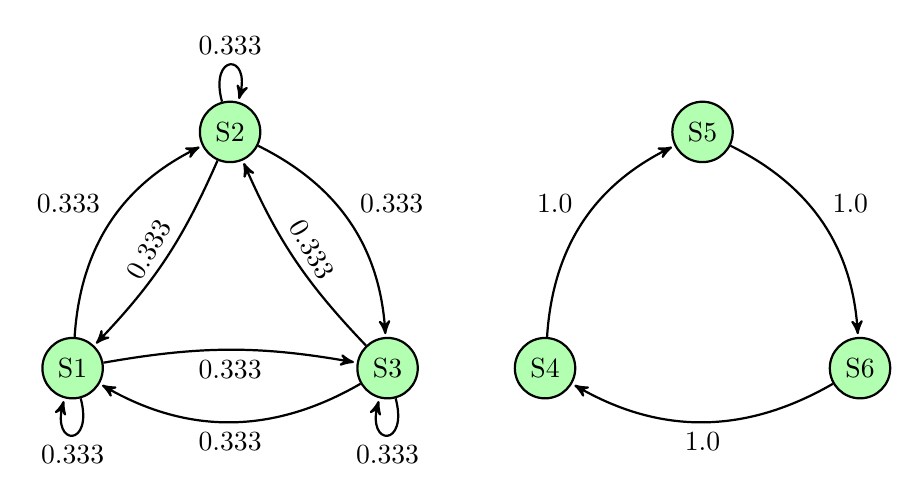
\begin{tikzpicture}[->,>=stealth',shorten >=1pt,auto,node distance=4cm,thick,main node/.style={circle,draw,font=\Large\bfseries}]
\tikzstyle{state} = [circle, draw=black, fill=green!30]
\tikzstyle{arrow} = [thick,->,>=stealth]

\node (s1) at (0,0) [state] {S1};
\node (s2) at (2,3) [state] {S2};
\node (s3) at (4,0) [state] {S3};
\node (s4) at (6,0) [state] {S4};
\node (s5) at (8,3) [state] {S5};
\node (s6) at (10,0) [state] {S6};

\path
    (s1) edge [loop below] node {0.333} (s1)
         edge [bend left] node {0.333} (s2)
         edge [bend left=10] node[below] {0.333} (s3)
    (s2) edge [loop above] node {0.333} (s2)
         edge [bend left=10] node[above,rotate=60] {0.333} (s1)
         edge [bend left] node {0.333} (s3)
    (s3) edge [loop below] node {0.333} (s3)
         edge [bend left=10] node[above,rotate=-60] {0.333} (s2)
         edge [bend left] node {0.333} (s1)
    (s4) edge [bend left] node {1.0} (s5)
    (s5) edge [bend left] node {1.0} (s6)
    (s6) edge [bend left] node {1.0} (s4);

\end{tikzpicture}
\caption{The graphical representation of our first model.}
\label{ref:nonmyo1}
\end{figure}

Figure \ref{ref:myoentropyfig} shows performance in terms of cumulative obtained reward for the
different methods proposed. The $h$ parameter determines the horizon of the particular solver. $h =
1$ results in a greedy solver. It is important to note that for POMCP and rPOMCP $h$ is merely an
upper bound on the depth of the decision tree they are allowed to explore. This is because they
build their decision tree incrementally, so that they may not reach its true bottom of their
decision tree if the number of samples is not sufficient.

\begin{figure}[ht!]
        \centering
        \begin{subfigure}[t]{0.45\textwidth}
                \includegraphics[width=\textwidth]{Images/MyoResults/1e4/E/output}
                \caption{Results using 1e4 samples, with entropy as the reward function.}
                \label{fig:m4e}
        \end{subfigure}%
        ~ %add desired spacing between images, e. g. ~, \quad, \qquad, \hfill etc.
          %(or a blank line to force the subfigure onto a new line)
        \begin{subfigure}[t]{0.45\textwidth}
                \includegraphics[width=\textwidth]{Images/MyoResults/1e4/MB/output}
                \caption{Results using 1e4 samples, with max-of-belief as the reward function.}
                \label{fig:m5e}
        \end{subfigure}
        \caption{Results in our first model, averaged over 3000 episodes.}
        \label{ref:myoentropyfig}
\end{figure}

We can see how a small horizon always results in a lower return over the 10 timesteps. This is
because with a greedy approach the agent cannot leverage the fact that half of the environment is
deterministic, and thus more useful to explore beforehand. This is most visible in the max-of-belief
setting, while the entropy reward function does not suffer from a significant loss of performance.

\section{Second Model - Finite Budget}

In this Section we apply the proposed algorithms to the following model: a 4-room world where a
target can transition, at each timestep, from a room to any of the two rooms adjacent. The
observation and reward function follow the logic of our first model: the agent can observe a single
room at a time, and needs to keep track of the target for 15 timesteps. The target here always
starts from a given room, known to the agent.

In this model there is an additional rule: the agent is only allowed to look at the world 4 times;
after that each action will yield no additional information. The agent can, at each timestep, decide
whether to use one of its observations, or save them for a future timestep. This last constraint is
used to simulate real-life resource constraints; for example when energy and/or processing
constraints limit the number of times a multi-camera system is allowed to observe the environment.

The idea is that the agent should use up an observation only if has low knowledge about the world;
otherwise it should keep its observation actions for later and try to extract as much reward from
current knowledge as possible.

\begin{figure}[ht]
\centering
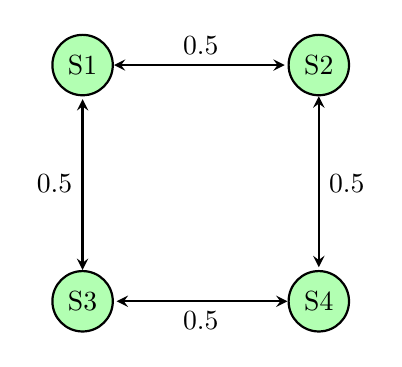
\begin{tikzpicture}[->,>=stealth',shorten >=1pt,auto,node distance=4cm,thick,main node/.style={circle,draw,font=\Large\bfseries}]
\tikzstyle{state} = [circle, draw=black, fill=green!30]
\tikzstyle{arrow} = [thick,<->,>=stealth]

\node (s1) at (0,3) [state] {S1};
\node (s2) at (3,3) [state] {S2};
\node (s3) at (0,0) [state] {S3};
\node (s4) at (3,0) [state] {S4};

\path
    (s1) edge [arrow] node {0.5} (s2)
    (s2) edge [arrow] node {0.5} (s4)
    (s3) edge [arrow] node {0.5} (s1)
    (s4) edge [arrow] node {0.5} (s3);

\end{tikzpicture}
\caption{The graphical representation of our second model.}
\label{ref:finbudget1}
\end{figure}

We tested this model in two configurations: one where the target transitions randomly between the
two rooms available, increasing maximally the entropy at each timestep, and one where the target
transitions to its left with a probability of $0.75$. This was done in order to see how the agent behavior
changed with respect to a differently predictable target.

\begin{figure}[ht]
        \centering
        \begin{subfigure}[t]{0.45\textwidth}
                \includegraphics[width=\textwidth]{Images/FiniteBudgetResults/0.5/1e4/E/output}
                \caption{Results using 1e4 samples, and entropy as the reward function.}
                \label{fig:fb4e5}
        \end{subfigure}%
        ~ %add desired spacing between images, e. g. ~, \quad, \qquad, \hfill etc.
          %(or a blank line to force the subfigure onto a new line)
        \begin{subfigure}[t]{0.45\textwidth}
                \includegraphics[width=\textwidth]{Images/FiniteBudgetResults/0.5/1e4/MB/output}
                \caption{Results using 1e4 samples, and max-of-belief as the reward function.}
                \label{fig:fb5e5}
        \end{subfigure}
        \caption{Results in the Finite Budget model with a transition factor of 0.5, averaged over 3000 episodes.}
        \label{ref:fbentropyfig5}
\end{figure}

\begin{figure}[ht]
        \centering
        \begin{subfigure}[t]{0.45\textwidth}
                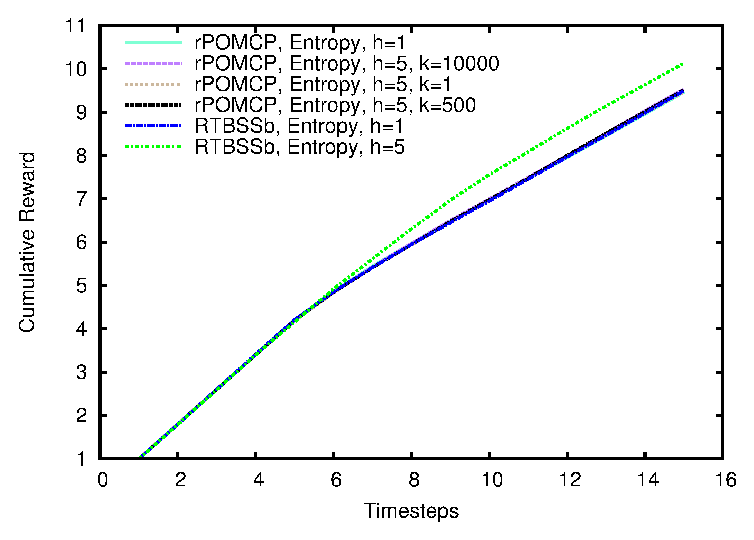
\includegraphics[width=\textwidth]{Images/FiniteBudgetResults/0.75/1e4/E/output}
                \caption{Results using 1e4 samples, and entropy as the reward function.}
                \label{fig:fb4e75}
        \end{subfigure}%
        ~ %add desired spacing between images, e. g. ~, \quad, \qquad, \hfill etc.
          %(or a blank line to force the subfigure onto a new line)
        \begin{subfigure}[t]{0.45\textwidth}
                \includegraphics[width=\textwidth]{Images/FiniteBudgetResults/0.75/1e4/MB/output}
                \caption{Results using 1e4 samples, and max-of-belief as the reward function.}
                \label{fig:fb5e75}
        \end{subfigure}
        \caption{Results in the Finite Budget model with a transition factor of 0.75, averaged over 3000 episodes.}
        \label{ref:fbentropyfig75}
\end{figure}

\section{Third Model - Realistic Scenario}

In this Section we test rPOMCP on yet another model. Here the target can walk in a grid world, in a
north-south-east-west fashion. To produce a somewhat realistic environment, the target selects a
random cell at any time, and then moves towards it. Once it reaches it, it selects another goal
cell, and continues. However, the agent's model of the environment does not include this: the agent
only knows that the target can move randomly towards an adjacent cell. The target always starts from
the center of the grid, with the agent knowing it.

The world is observed by cameras, where each camera can observe a 5x5 patch of the overall world.
Each camera can observe imperfectly: the closer the target is towards the center of the patch, the
more accurate the observations will be. Otherwise the camera will report the target on any cell
adjacent to the true target. If the reported cell is outside the camera range, the camera will not
report observing the target.

The agent is allowed to use a single camera at the time, and again needs to keep track of the target
over 75 timesteps.

We show results with two different versions of the world: a small 20x20 environment, and a bigger
50x50 one. Due to the big number of states, POMCP and RTBSS cannot be used here; RTBSSb can be
barely used with a greedy horizon for the small environment.

\begin{figure}[ht]
        \centering
        \begin{subfigure}[t]{0.45\textwidth}
                \includegraphics[width=\textwidth]{Images/CameraBasicResults/Small_20x20/1e4/output}
                \caption{Results using 1e4 samples.}
                \label{fig:cws4mb}
        \end{subfigure}%
        ~ %add desired spacing between images, e. g. ~, \quad, \qquad, \hfill etc.
          %(or a blank line to force the subfigure onto a new line)
        \begin{subfigure}[t]{0.45\textwidth}
                \includegraphics[width=\textwidth]{Images/CameraBasicResults/Big_50x50/1e4/output}
                \caption{Results using 1e5 samples.}
                \label{fig:cws5mb}
        \end{subfigure}
        \caption{Results in our realistic model using a 20x20 grid, using max-of-belief, averaged over 3000 episodes.}\label{fig:cwsmb}
\end{figure}

In Figure \ref{fig:cwb10} we show the results of applying rPOMCP to a multi-tracking scenario, where
10 targets are allowed to roam the grid world concurrently. In this experiment, we run 10 instances
of rPOMCP in a parallel fashion, one for each target. These 10 instances approximate values for
every possible action, given their belief on their respective target. At every timestep, the action that
maximizes overall value over all rPOMCP instances is chosen.

\begin{figure}[ht!]
        \centering
        \begin{subfigure}[t]{0.5\textwidth}
                \includegraphics[width=\textwidth]{Images/CameraBasicResults/Big_50x50/Multi/E/output}
                \caption{Results using 1e4 samples and entropy.}
                \label{fig:cwb4e10}
        \end{subfigure}%
        ~ %add desired spacing between images, e. g. ~, \quad, \qquad, \hfill etc.
          %(or a blank line to force the subfigure onto a new line)
        \begin{subfigure}[t]{0.5\textwidth}
                \includegraphics[width=\textwidth]{Images/CameraBasicResults/Big_50x50/Multi/MB/output}
                \caption{Results using 1e4 samples and max-of-belief.}
                \label{fig:cwb5mb10}
        \end{subfigure}
        \caption{Results in our realistic model 50x50 tracking 10 unique targets, averaged over 3000 episodes.}\label{fig:cwb10}
\end{figure}

In addition to the previous experiments, we also created a separate model where the agent's model of
the target movements is improved. In this second version of Camera World, the model keeps track of
the previous direction that the target moved, and predicts a $0.7$ probability that the target will
continue to move in the same direction, or randomly otherwise. This is done by increasing the state
space by four times, where each state now encodes a previous target direction and the target current
position.

In this new model unfortunately RTBSSb cannot be used, as the state space is too big and RTBSSb
takes too much time to complete.

\begin{figure}[ht!]
        \centering
        \begin{subfigure}[t]{0.45\textwidth}
                \includegraphics[width=\textwidth]{Images/CameraPathResults/Small_20x20/1e4/output}
                \caption{Results using 1e4 samples.}
                \label{fig:cps4e}
        \end{subfigure}%
        ~ %add desired spacing between images, e. g. ~, \quad, \qquad, \hfill etc.
          %(or a blank line to force the subfigure onto a new line)
        \begin{subfigure}[t]{0.45\textwidth}
                \includegraphics[width=\textwidth]{Images/CameraPathResults/Big_50x50/1e4/output}
                \caption{Results using 1e5 samples.}
                \label{fig:cps5e}
        \end{subfigure}
        \caption{Results in the Camera World 2 20x20, using entropy, averaged over 3000 episodes.}\label{fig:cpse}
\end{figure}

\begin{figure}[ht]
        \centering
        \begin{subfigure}[t]{0.5\textwidth}
                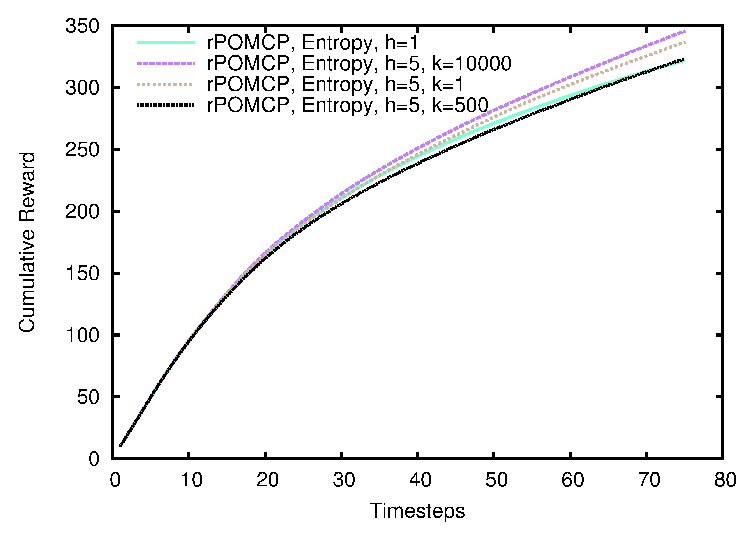
\includegraphics[width=\textwidth]{Images/CameraPathResults/Big_50x50/Multi/E/output}
                \caption{Results using 1e4 samples and entropy.}
                \label{fig:cpb4e10}
        \end{subfigure}%
        ~ %add desired spacing between images, e. g. ~, \quad, \qquad, \hfill etc.
          %(or a blank line to force the subfigure onto a new line)
        \begin{subfigure}[t]{0.5\textwidth}
                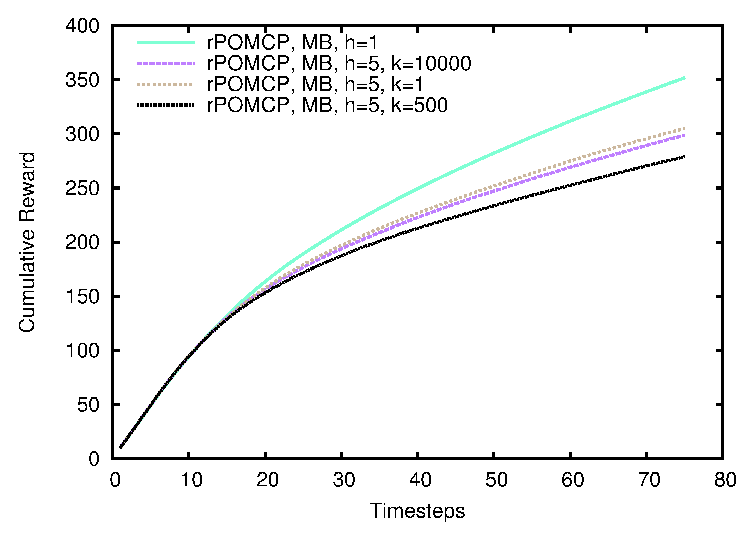
\includegraphics[width=\textwidth]{Images/CameraPathResults/Big_50x50/Multi/MB/output}
                \caption{Results using 1e4 samples and max-of-belief.}
                \label{fig:cpb5mb10}
        \end{subfigure}
        \caption{Results in the Camera World 2 50x50 tracking 10 unique targets, averaged over 3000 episodes.}\label{fig:cpb10}
\end{figure}


\chapter{Conclusion}\label{ref:conclusion}
In this thesis we tackle Active Perception for resource allocation in multi-camera systems. In
particular, we try to track a number of targets over an extended period of time, while trying to make an
optimal usage of available resources under specific constraints, namely partial
observability, environment size and limited access to cameras.

In order to fulfill our goal we have improved over an existing approach in order to fit our particular
prerequisites, removing shortcomings which prevented its application in our setting. Starting from the POMCP algorithm, which uses online Monte Carlo techniques to
approximately plan in POMDP models, we have extended it in order to be applied to belief-based
POMDPs, called $\rho$POMDPs, using entropy or max-of-belief as reward functions. Our approach,
called $\rho$-POMCP, can tackle problems orders of magnitude bigger than existing alternatives and
can be applied to all $\rho$POMDP problems, not only those proposed in this work.

$\rho$-POMCP achieves these results by estimating the belief-based reward function directly on the particle beliefs, without the need for full beliefs to be propagated within the search tree. In addition each updated estimate can be cheaply backpropagated up in the tree substituting previous estimates, guaranteeing that the UTC process always uses the most current available information in order to select the best available action. The method does not require significant additional computation with respect to the original method POMCP, which allows it to be applied to large sized problems.

We have compared our approach to already existing methods, and shown the differences in performance
between them. In particular, $\rho$-POMCP can scale successfully on problems orders of magnitude
bigger than what was possible with previous approaches, and can be used to track multiple targets
concurrently in a very effective and parallelizable manner. In particular, our approach can be
easily distributed between separate computing nodes, and the amount of information and bandwidth
that needs to be shared between any such nodes is very limited.

At the same time, our results indicate that while theoretically non-myopic solutions are sometimes
necessary for optimal solutions in Active Perception, in a multi-camera system setting the added
overhead required by planning over more than a single timestep may not be justified by the
additional gained rewards - if the model of the environment even allows for any. This seems to
replicate results obtained by \cite{cit:relworktanks}, which show that planning for more than one timestep in a realistic
setting does not seem to improve effectiveness much, while it is needed when the problem is
artificially constrained so to require forethinking by the agent.

\section{Future Work}

Additional efforts may be useful in order to evaluate the effectiveness of our method on
$\rho$POMDPs where actions actually do influence the environment. In such cases the value in
planning for the future and avoid myopicity is increased as the agent's actions need to be selected
taking into consideration how the environment will change with respect to the agent's choice.

Another improvement would be to extend our reward approximations with respect to reward functions
other than entropy and max-of-belief.


\nocite{*}
\appendix

\chapter{Myopicity of Active Perception}\label{ref:appendix_proof}
POMDPs can be used naturally to compute non-myopic policies to solve a particular task. We show here
that some active perception tasks require the usage of non-myopic solutions to achieve optimality,
and thus we can use POMDPs to model efficiently such tasks.

We propose two different POMDP models of active perception problems. For one of the models we will
prove that a non-myopic solution is required in order to obtain an optimal solution. For the second
we will prove that a non-myopic solution is not required. The results we show are for both max of
belief and negative entropy reward functions.

\section{Non-Myopic Solution}

Let's consider a world where the agent is tasked with tracking a single person that is walking. The
person can, at any moment, be in one of a series of rooms, and can transition between them. In each
room there is a camera which can observe the room itself and nothing else. If the agent activates
the camera situated in a room the person just entered there is a $0.8$ probability that the agent will
obtain a ``found'' observation, and a $0.2$ probability that it will obtain a ``null'' observation.
On the other hand, if the agent activates any other camera, it will obtain a ``null'' observation
with $0.8$ probability and a ``found'' observation with $0.2$ probability. At each timestep
the person will move to another accessible room, and then the agent will activate a single camera.
The agent's goal is to guess correctly where the person has moved for two times in a row, knowing
only that at the start the person could be in any room.

We will now create an instance of the problem we have just finished describing. Let's now suppose
that in our world there are 6 rooms, and we know that the person will transition from one to another
with the following probabilities:

\begin{center}
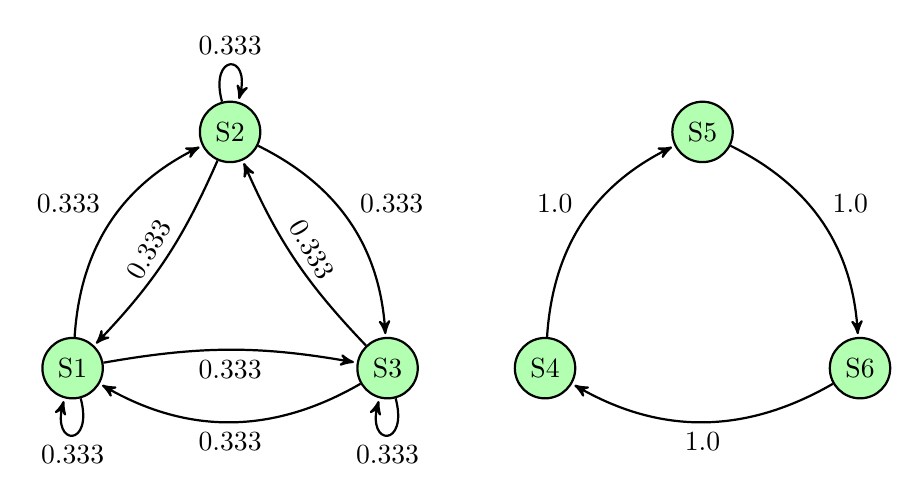
\begin{tikzpicture}[->,>=stealth',shorten >=1pt,auto,node distance=4cm,thick,main node/.style={circle,draw,font=\Large\bfseries}]
\tikzstyle{state} = [circle, draw=black, fill=green!30]
\tikzstyle{arrow} = [thick,->,>=stealth]

\node (s1) at (0,0) [state] {S1};
\node (s2) at (2,3) [state] {S2};
\node (s3) at (4,0) [state] {S3};
\node (s4) at (6,0) [state] {S4};
\node (s5) at (8,3) [state] {S5};
\node (s6) at (10,0) [state] {S6};

\path
    (s1) edge [loop below] node {0.333} (s1)
         edge [bend left] node {0.333} (s2)
         edge [bend left=10] node[below] {0.333} (s3)
    (s2) edge [loop above] node {0.333} (s2)
         edge [bend left=10] node[above,rotate=60] {0.333} (s1)
         edge [bend left] node {0.333} (s3)
    (s3) edge [loop below] node {0.333} (s3)
         edge [bend left=10] node[above,rotate=-60] {0.333} (s2)
         edge [bend left] node {0.333} (s1)
    (s4) edge [bend left] node {1.0} (s5)
    (s5) edge [bend left] node {1.0} (s6)
    (s6) edge [bend left] node {1.0} (s4);

\end{tikzpicture}
\end{center}

As we said, at first the agent does not know where the person is at all. The myopic expected return
for the first step only is:

\[ E[\text{return}| a_1 ] = \sum_{o\in \Omega} p(o | b, a_1) \cdot \rho(b') \]

Where $b'$ is the result of the belief update of $b$ with $o$ and $a_1$. The non-myopic expected return over
both steps is:

\[ E[\text{return}| a_1, a_2] = \sum_{o \in \Omega} p(o | b, a_1) \left ( \rho(b') + \sum_{o' \in
\Omega} p(o'| b', a_2) \cdot \rho(b'') \right ) \]

Where $b''$ updates from $b'$, $o'$ and $a_2$. It is easy to show that, both for max of belief and
negative entropy as $\rho$, all actions in the presented problem have the same myopic one-step
expected return from a uniform belief. This is done by simply computing the previously described
summatory over every term and performing the appropriate belief updates.

However, expected non-myopic returns are not the same for all choices of $a_1$ and $a_2$. For
example selecting $a_1 = S1$ always results in a certain expected return $v$, independently from
$a_2$. On the other hand, if $a_1 = S4$, all expected returns are greater than $v$ for all but one
choice of $a_2$. In other words, selecting $a_1 = S1$ leads necessarily to a lower two-step expected
return, since the agent can select $a_2$ to only pick the best cases.

Selecting $a_1$ to avoid the worst cases can only be done when there is a way to distinguish between
two different $a_1$.  Since myopic expected returns are the same for all $a_1$, this is impossible
to do with a myopic solution.

Note that the problem considered can be extended into uncountably many models where the same
properties apply. This could be done for example by adding a certain number of rooms that the person
needs to go through before ending up in the model presented, and so on. Thus a non-myopic solution
is required for uncountably many active perception tasks.

\section{Myopic Solution}

A different instance of the previous problem is one where there are only 4 rooms, and the person
will transition from state to state with the following probabilities:

\begin{center}
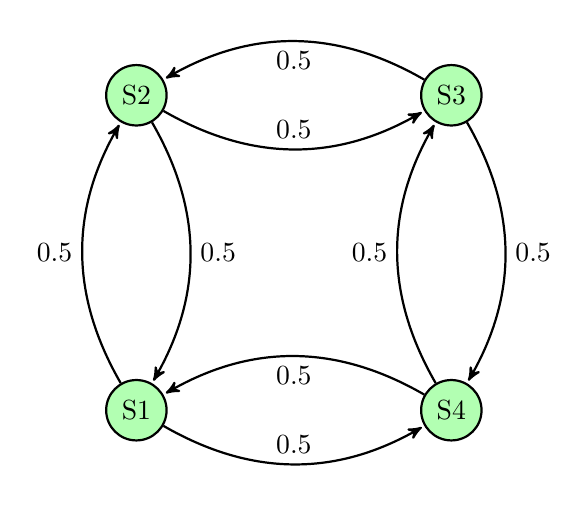
\begin{tikzpicture}[->,>=stealth',shorten >=1pt,auto,node distance=4cm,thick,main node/.style={circle,draw,font=\Large\bfseries}]
\tikzstyle{state} = [circle, draw=black, fill=green!30]
\tikzstyle{arrow} = [thick,->,>=stealth]

\node (s1) at (0,0) [state] {S1};
\node (s2) at (0,4) [state] {S2};
\node (s3) at (4,4) [state] {S3};
\node (s4) at (4,0) [state] {S4};

\path
    (s1) edge [bend right] node {0.5} (s4)
         edge [bend left] node {0.5} (s2)
    (s2) edge [bend left] node {0.5} (s1)
         edge [bend right] node {0.5} (s3)
    (s3) edge [bend right] node {0.5} (s2)
         edge [bend left] node {0.5} (s4)
    (s4) edge [bend left] node {0.5} (s3)
         edge [bend right] node {0.5} (s1);

\end{tikzpicture}
\end{center}

Once again, we can compute both myopic and non-myopic expected returns. This time, no matter the
choice of actions, there is no particular incentive for an agent to select a pair over another. If
$\rho$ is negative entropy, certain pair of actions have a higher expected return than others. But
for each $a_1$ there is a $a_2$ which obtains the maximum expected return possible.

Thus, non-myopic in this particular model has no particular advantage over a more simple myopic
solution. Once again this problem can be extended into uncountably infinite examples of active
perception tasks.



\bibliographystyle{unsrtnat}
\bibliography{references}

\end{document}
